\documentclass[11pt,a4paper]{article}

\usepackage[margin=2.4cm]{geometry}
\usepackage{amsmath,amssymb}
\usepackage{graphicx}
\usepackage{booktabs}
\usepackage[labelsep=period,font=small]{caption}
\usepackage[round]{natbib}
\usepackage{listings}
\usepackage{xcolor}
\usepackage{microtype}
\usepackage[colorlinks=true,linkcolor=black,citecolor=black,urlcolor=blue!70!black]{hyperref}

\graphicspath{{../figures/}}

\lstset{
  language=Python,
  basicstyle=\ttfamily\footnotesize,
  keywordstyle=\bfseries,
  commentstyle=\itshape\color{black!60},
  breaklines=true,
  frame=single,
  columns=fullflexible,
  showstringspaces=false
}

\newcommand{\E}{\mathbb{E}}

\begin{document}

\begin{center}
{\LARGE\bfseries Feynman-Kac in practice: when do grids beat Monte Carlo?\par}
\vspace{0.8em}
{\large Connor Mcareavey\par}
\vspace{0.3em}
COSC2500 Numerical Methods in Computational Science, project report, Semester 2, 2026\par
\vspace{0.3em}
\href{https://github.com/ConnorMcareavey/feynman-kac-option-pricing}{GitHub repository}
\end{center}

\begin{abstract}
\noindent The price of a European option in the Black-Scholes model is both the solution of a parabolic partial differential equation and an expectation over random stock price paths, a duality expressed by the Feynman-Kac formula. We use this to compare grid methods and Monte Carlo methods on problems with exact answers, so that every error reported is a true error. For the PDE we reduce the Black-Scholes equation to the heat equation and compare the explicit, implicit and Crank-Nicolson schemes. With practical time steps Crank-Nicolson fails to converge for a digital option, and we find that the standard two step Rannacher start-up restores the price but not the gamma, which needs four steps. For Monte Carlo we separate the statistical error from the Euler-Maruyama bias using coupled simulations. We then derive and measure how both approaches scale with the number of underlying assets, and find a crossover at about four to five dimensions for tensor product quadrature and about three for a time stepping PDE solver. An extension prices baskets of up to 20 correlated stocks, where a geometric basket control variate reduces the variance by factors of 25 to over 2000.
\end{abstract}

\section{Introduction}

Mathematical models are only useful in computational science if they can be turned into numbers. For the simplest model of a stock price, the Black-Scholes model, the price of a European option can be written in closed form. For almost anything more realistic it cannot, and a numerical method is needed. There are two quite different families of methods. The first solves a partial differential equation for the option price on a grid. The second simulates many random paths of the stock and averages the payoff. The Feynman-Kac formula guarantees that both compute the same number, but they have very different error behaviour and very different costs.

This report asks when each approach should be used. We work throughout with problems that have exact answers, namely a European call, a cash-or-nothing digital call and a geometric basket option, so that every error is measured against the truth rather than estimated. Section~\ref{sec:background} states the model and the Feynman-Kac connection and reviews previous work. Section~\ref{sec:pde} solves the PDE by finite differences, with particular attention to stability and to the loss of accuracy near the strike, where the payoffs are not smooth. Section~\ref{sec:mc} prices the same option by Monte Carlo and separates the statistical error from the bias of Euler-Maruyama time stepping. Section~\ref{sec:dim} derives how the cost of each method grows with the number of underlying assets and measures the crossover on a problem with an exact price in every dimension. Section~\ref{sec:basket} applies this to a basket of up to 20 correlated stocks. Sections~\ref{sec:vv} to~\ref{sec:conclusions} cover verification and validation, the practical meaning of the results, their limitations and our conclusions, and Section~\ref{sec:self} gives a self-assessment against the marking criteria.

The project draws on every module of the course \citep{notes2026}. The finite difference formulas and the trouble caused by discontinuities come from Module 1, banded linear systems and the Cholesky factorisation from Module 2, time stepping and stiffness from Module 3, and PDEs, Monte Carlo methods, stochastic differential equations and error estimation from Module 4. Sections of the course notes are cited as, for example, Notes~4.9, to distinguish them from sections of this report. All code is written in Python, every random number comes from a seeded generator, and every figure can be regenerated from the notebooks in the repository linked above.

\section{Background}\label{sec:background}

\subsection{The Black-Scholes model and the Feynman-Kac formula}

In the Black-Scholes model the stock price $S$ follows geometric Brownian motion under the risk neutral measure,
\begin{equation}
dS = rS\,dt + \sigma S\,dB_t, \label{eq:gbm}
\end{equation}
where $r$ is the risk free interest rate, $\sigma$ the volatility and $B_t$ a standard Brownian motion. A European option pays $f(S(T))$ at the expiry time $T$. Its value $V(S,t)$ satisfies the Black-Scholes equation
\begin{equation}
\frac{\partial V}{\partial t} + \frac{1}{2}\sigma^2S^2\frac{\partial^2V}{\partial S^2} + rS\frac{\partial V}{\partial S} - rV = 0, \qquad V(S,T) = f(S), \label{eq:bs}
\end{equation}
and it is also the discounted expected payoff
\begin{equation}
V(S,t) = e^{-r(T-t)}\,\E\left[f(S(T)) \mid S(t) = S\right]. \label{eq:fk}
\end{equation}
The Feynman-Kac theorem states that \eqref{eq:bs} and \eqref{eq:fk} define the same function, and the idea of the proof is short. If $V$ solves \eqref{eq:bs}, It\^o's formula applied to $Y_t = e^{-rt}V(S(t),t)$ gives
\begin{equation}
dY_t = e^{-rt}\left(\frac{\partial V}{\partial t} + \frac{1}{2}\sigma^2S^2\frac{\partial^2V}{\partial S^2} + rS\frac{\partial V}{\partial S} - rV\right)dt + e^{-rt}\sigma S\frac{\partial V}{\partial S}\,dB_t.
\end{equation}
The bracket vanishes by \eqref{eq:bs}, so $Y_t$ is a stochastic integral with zero mean under mild conditions on $V$, and $\E[Y_T] = Y_0$ is exactly \eqref{eq:fk} at $t = 0$.

Equation \eqref{eq:bs} leads to grid methods, whose errors come from the grid spacing and whose main risks are instability and loss of accuracy where the payoff is not smooth. Equation \eqref{eq:fk} leads to Monte Carlo, whose errors come from the finite number of paths and from time stepping. Throughout the report we use $S_0 = K = 100$, $r = 0.05$, $\sigma = 0.2$ and $T = 1$. The two single stock options are a European call with payoff $\max(S - K, 0)$, worth $10.4506$, and a cash-or-nothing digital call paying 1 if $S > K$, worth $0.5323$. The call payoff has a kink at the strike and the digital payoff a jump, and both cause the same kind of difficulty that discontinuities cause for numerical integration in exercise R1.3.

\subsection{Previous work}

The Black-Scholes equation was derived by \citet{black1973} and \citet{merton1973} from a hedging argument. A portfolio of the option and the stock can be made riskless, so it must earn the risk free rate. Writing the solution as an expectation is an older idea. \citet{feynman1948} expressed solutions of the Schr\"odinger equation as averages over paths, and \citet{kac1949} made the corresponding result for the heat equation rigorous, which is the origin of the name Feynman-Kac. In finance the expectation form is the risk neutral pricing formula \eqref{eq:fk}.

Finite difference methods were applied to option pricing from the late 1970s, with \citet{brennan1978} giving an early systematic treatment. The scheme of \citet{crank1947}, developed for heat conduction, became the standard choice because it is second order and unconditionally stable, and the change of variables to the heat equation used in Section~\ref{sec:pde} is the classical one presented by \citet{wilmott1995}. The weakness of Crank-Nicolson with non-smooth data was identified by \citet{rannacher1984} for parabolic equations in general. His remedy of a few implicit start-up steps was studied for option payoffs by \citet{pooley2003} and analysed by \citet{giles2006}. Section~\ref{sec:pde} reproduces their main observations and adds a measurement of how many start-up steps the gamma of a digital option needs.

The Monte Carlo method goes back to \citet{metropolis1949}, and \citet{boyle1977} first used it to price options. The standard modern reference is \citet{glasserman2004}, which covers variance reduction methods such as the geometric average control variate of \citet{kemna1990} used in Section~\ref{sec:basket}. The Euler-Maruyama method is named after \citet{maruyama1955}, and \citet{higham2001} gives an accessible account of its weak and strong orders of convergence. \citet{duffie1995} showed how a fixed computing budget should be divided between time steps and paths, which leads to the $\varepsilon^{-3}$ cost measured in Section~\ref{sec:mc}, and the multilevel method of \citet{giles2008} was designed to bring that cost back towards $\varepsilon^{-2}$.

The phrase ``curse of dimensionality'' is due to \citet{bellman1957}. The comparison between a grid's error of order $n^{-2/d}$ and Monte Carlo's $n^{-1/2}$ is standard \citep[Section 1.1]{glasserman2004}, and it is the usual reason given for pricing multi-asset products by simulation. Sparse grids \citep{bungartz2004} reduce the number of points a grid needs from about $n^d$ to about $n(\log n)^{d-1}$ for sufficiently smooth functions, which pushes the crossover to higher dimensions, although payoffs with kinks are exactly the functions that are not smooth enough for the full benefit. What this project adds is a direct measurement of the crossover on a problem with an exact answer in every dimension, including the extra cost of time stepping in a PDE solver and the effect of the explicit scheme's stability limit.

\section{Finite difference solution of the PDE}\label{sec:pde}

\subsection{Reduction to the heat equation}

Following \citet{wilmott1995} we set $S = Ke^x$, $t = T - 2\tau/\sigma^2$ and $V = Kv(x,\tau)$, so that $x = \ln(S/K)$ and $\tau = \frac{1}{2}\sigma^2(T-t)$ is a rescaled time to expiry. The chain rule gives $SV_S = Kv_x$ and $S^2V_{SS} = K(v_{xx} - v_x)$, and substituting into \eqref{eq:bs} gives the constant coefficient equation
\begin{equation}
v_\tau = v_{xx} + (k-1)v_x - kv, \qquad k = \frac{2r}{\sigma^2}.
\end{equation}
Writing $v = e^{\alpha x + \beta\tau}u$ and cancelling the common exponential factor gives
\begin{equation}
u_\tau = u_{xx} + (2\alpha + k - 1)u_x + \left(\alpha^2 + (k-1)\alpha - k - \beta\right)u,
\end{equation}
so the choices $\alpha = -\frac{1}{2}(k-1)$ and $\beta = -\frac{1}{4}(k+1)^2$ remove both lower order terms and leave the heat equation
\begin{equation}
u_\tau = u_{xx}. \label{eq:heat}
\end{equation}
The Black-Scholes equation run backwards from expiry is therefore the heat equation run forwards in $\tau$, with the payoff as the initial condition $u(x,0) = e^{-\alpha x}f(Ke^x)/K$. For the call this is $\max(e^{(k+1)x/2} - e^{(k-1)x/2}, 0)$. We solve on $-2 \le x \le 2$, which covers $13.5 \le S \le 739$. At the lower boundary $V = 0$, and at the upper boundary we impose the deep in the money values $V = S - Ke^{-r(T-t)}$ for the call and $V = e^{-r(T-t)}$ for the digital, converted to $u$ by the same substitution. With a fixed grid spacing the price at the strike was unchanged to about $10^{-12}$ for every $x_{\max} \ge 1$, so the truncation of the domain is negligible. At a node lying exactly on the strike, the digital payoff is given the average of its one-sided limits, $\frac{1}{2}$.

The factor $e^{\alpha x + \beta\tau}$ can be large, but multiplication preserves relative error, so it causes no cancellation of the kind described in Notes~1.1.1. The real risk is overflow (Notes~1.1.3). The largest exponent is about $\frac{1}{2}(k+1)x_{\max}$, which is $3.5$ for our parameters but passes the double precision limit of about 709 once $\sigma$ falls to about 1\%, and the solver does indeed fail there. A more important limitation is that the transformation needs constant $r$ and $\sigma$.

\subsection{The theta scheme and its stability}

On a uniform grid $x_j$, $\tau_n$ with mesh ratio $\lambda = \Delta\tau/\Delta x^2$, the theta scheme for \eqref{eq:heat} is
\begin{equation}
u_j^{n+1} - u_j^n = \lambda\theta\,\delta^2u_j^{n+1} + \lambda(1-\theta)\,\delta^2u_j^n, \qquad \delta^2u_j = u_{j-1} - 2u_j + u_{j+1}. \label{eq:theta}
\end{equation}
With $\theta = 0$ this is the explicit forward difference method of Sauer's Program~8.1 \citep{sauer2018}, with $\theta = 1$ the implicit backward difference method, and with $\theta = \frac{1}{2}$ the Crank-Nicolson method. The local truncation error is $O(\Delta\tau + \Delta x^2)$ unless $\theta = \frac{1}{2}$, when it is $O(\Delta\tau^2 + \Delta x^2)$, for the same reason that the central difference of Notes~1.3.3 is second order. For $\theta > 0$ each step requires the solution of a tridiagonal system, and since this is a banded system (Notes~2.3.8) it costs only $O(N_x)$ operations with \texttt{scipy.linalg.solve\_banded}.

A von Neumann analysis substitutes the Fourier mode $u_j^n = g^ne^{\mathrm{i}j\xi\Delta x}$ into \eqref{eq:theta}. Writing $s = \sin^2(\frac{1}{2}\xi\Delta x)$, the amplification factors of the three schemes are
\begin{equation}
g_{\mathrm{exp}} = 1 - 4\lambda s, \qquad g_{\mathrm{imp}} = \frac{1}{1 + 4\lambda s}, \qquad g_{\mathrm{CN}} = \frac{1 - 2\lambda s}{1 + 2\lambda s}. \label{eq:amp}
\end{equation}
The explicit scheme is stable only for $\lambda \le \frac{1}{2}$, which in calendar time is $\Delta t \le \Delta x^2/\sigma^2$. The same condition explains exercise R4.1(a), where $u_t = 2u_{xx}$ with $h = 0.1$ requires $k \le 0.0025$. The other two schemes are unconditionally stable, but they treat the sawtooth mode $s = 1$, the mode most strongly excited by a kink or jump in the payoff, very differently. As $\lambda \to \infty$ the implicit factor tends to 0, while the Crank-Nicolson factor tends to $-1$, so high frequency errors flip sign every step and decay very slowly. In the language of Notes~3.4 these modes are the stiff components of the semi-discrete system, and Crank-Nicolson is A-stable but not L-stable. The standard remedy, due to \citet{rannacher1984}, is to take the first few steps with $\theta = 1$ before switching to Crank-Nicolson.

\subsection{Stability in practice}

Just below the limit, at $\lambda = 0.48$ on 200 intervals, the explicit scheme has a largest error of $8.2\times10^{-3}$. Just above it, at $\lambda = 0.52$, the sawtooth mode grows by a factor $|1 - 4\lambda| \approx 1.08$ per step, and after 96 steps the largest error is 43. The heat equation coordinates also make this limit independent of the extent of the grid. In the original variable $S$ on a grid $S_j = j\Delta S$, the explicit update has diagonal coefficient $b_j = 1 - \Delta t(\sigma^2j^2 + r)$, so keeping it non-negative at the top node needs roughly $\Delta t \le 1/(\sigma^2N_S^2 + r)$ with $N_S = S_{\max}/\Delta S$. Figure~\ref{fig:stabgrid} compares this bound with the largest stable step found by bisection, using $\Delta S = 1$ and $\Delta x = 0.01$, which give the same resolution at the strike. In $S$ the limit falls like $1/S_{\max}^2$, so raising $S_{\max}$ from 200 to 800 needs 17 times as many steps. In $x$ it stays at $\lambda \approx 0.51$ for grids reaching up to $S_{\max} = 5460$.

\begin{figure}[htbp]
\centering
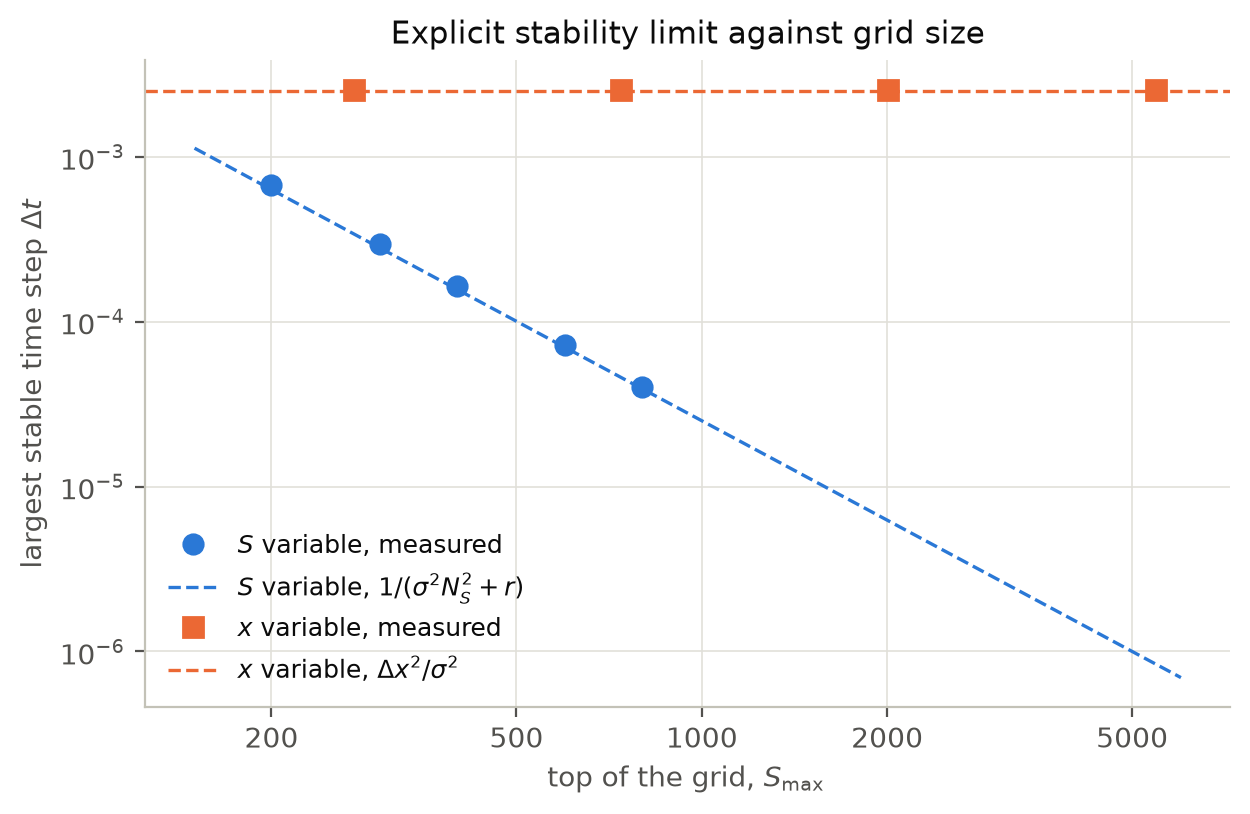
\includegraphics[width=0.62\textwidth]{01_stability_vs_grid_size.png}
\caption{Largest stable explicit time step against the top of the grid. In the original variable $S$ the limit follows $1/(\sigma^2N_S^2 + r)$ and shrinks like $1/S_{\max}^2$. In the log variable $x$ it is fixed by $\lambda \le \frac{1}{2}$, whatever the size of the grid.}
\label{fig:stabgrid}
\end{figure}

\subsection{Convergence and the non-smooth payoff problem}

Figure~\ref{fig:conv} and Table~\ref{tab:orders} compare the four schemes as the grid is refined. For the implicit methods we tie the time step to the space step with $N_\tau = N_x/40$, which corresponds to one step per 0.1 years on the coarsest grid, typical of practice, and gives $\lambda$ between 20 and 320. The explicit scheme cannot use such steps and keeps $\lambda = 0.4$. The error is the largest absolute error over $80 < S < 125$. Measuring only at $S = K$ hides part of the problem, because the oscillations described below partly cancel at the strike node by symmetry.

\begin{figure}[htbp]
\centering
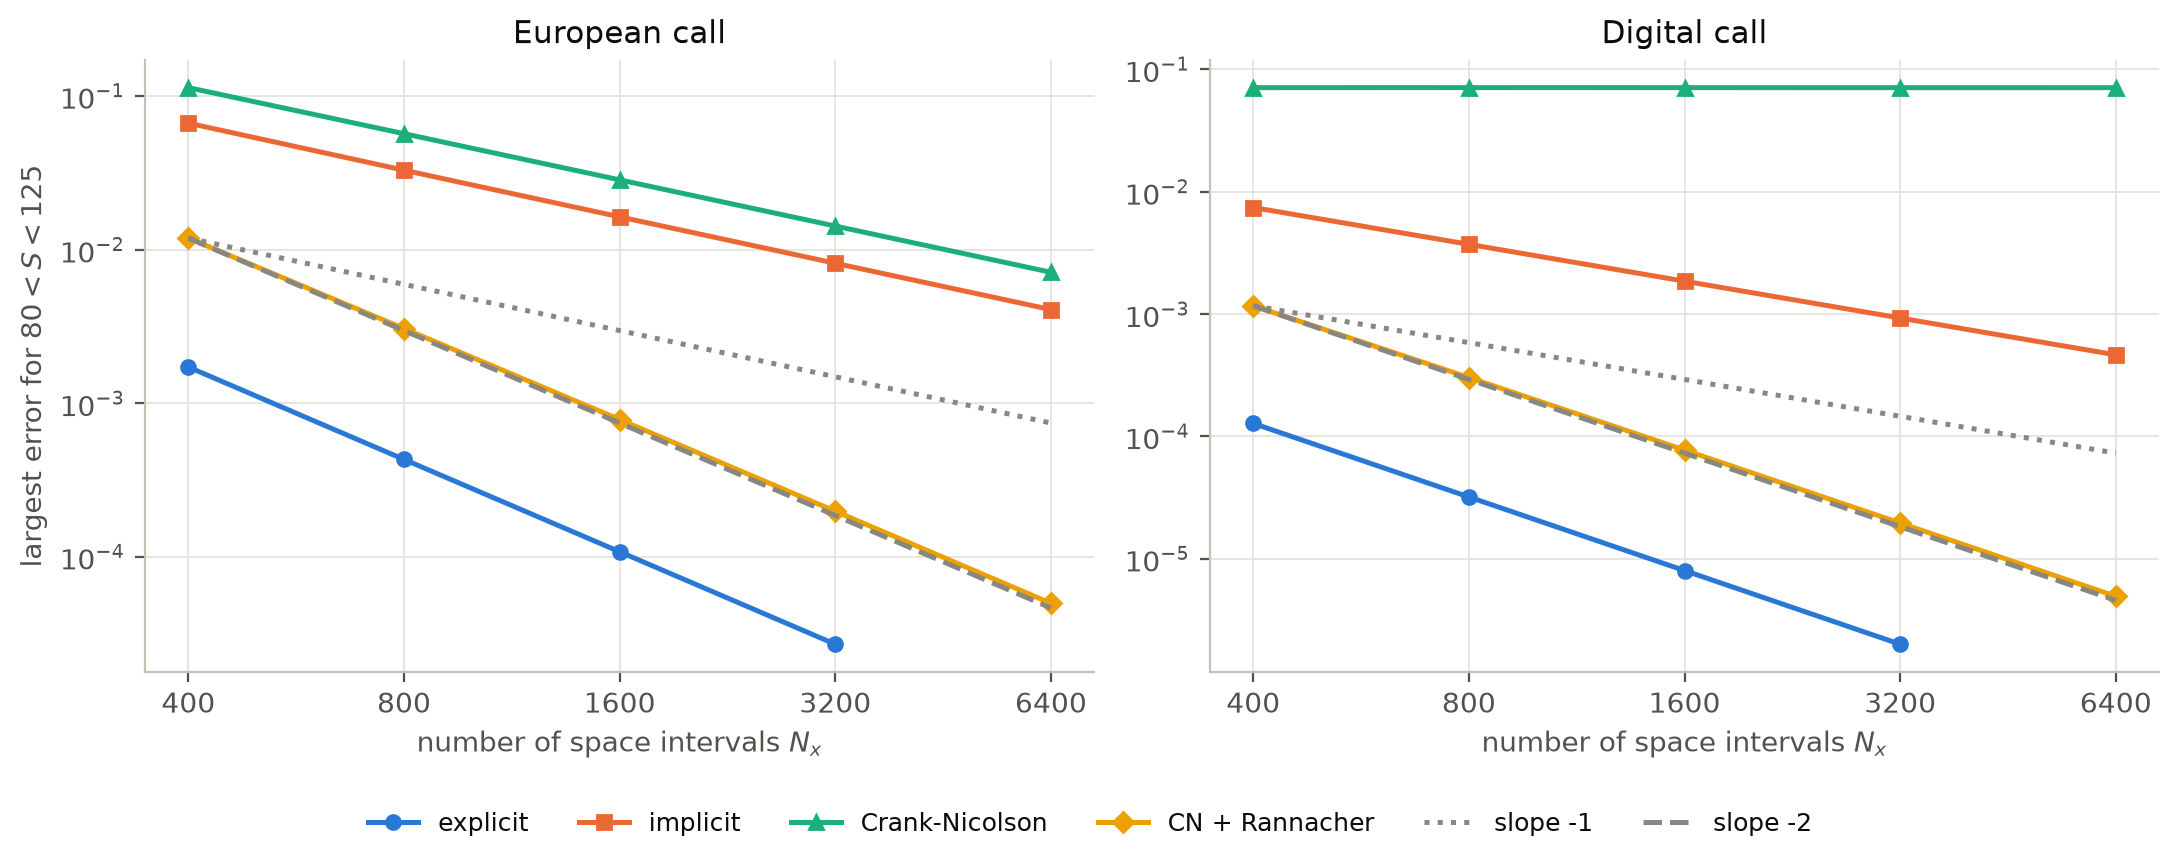
\includegraphics[width=\textwidth]{01_convergence.png}
\caption{Largest error over $80 < S < 125$ against the number of space intervals, with $N_\tau = N_x/40$ for the implicit methods and $\lambda = 0.4$ for the explicit scheme. Plain Crank-Nicolson is first order for the call and does not converge for the digital.}
\label{fig:conv}
\end{figure}

\begin{table}[htbp]
\centering
\caption{Observed orders of convergence of the largest error over $80 < S < 125$, between the two finest grids computed.}
\label{tab:orders}
\begin{tabular}{llcc}
\toprule
Scheme & Time step & Call & Digital \\
\midrule
Explicit & $\lambda = 0.4$ & 2.00 & 2.00 \\
Implicit & $N_\tau = N_x/40$ & 1.00 & 1.00 \\
Crank-Nicolson & $N_\tau = N_x/40$ & 1.00 & 0.00 \\
Crank-Nicolson with two Rannacher steps & $N_\tau = N_x/40$ & 1.99 & 1.99 \\
\bottomrule
\end{tabular}
\end{table}

The explicit scheme converges at second order but its cost grows like $N_x^3$, and the implicit scheme is held to first order by its $O(\Delta\tau)$ error. Crank-Nicolson, which should be second order, is first order for the call, and for the digital its error stays at 0.071 however fine the grid. With two Rannacher steps both options converge cleanly at second order, so the failure is not a coding error. Figure~\ref{fig:osc} shows what goes wrong on a grid with $N_x = 800$ and $N_\tau = 20$, so that $\lambda = 40$. The Crank-Nicolson digital price zigzags around the exact curve near the strike with errors up to 0.07. The call price looks correct, but its gamma has an error of 0.6 at the strike, about thirty times the true value of 0.019. A kink leaves high frequency errors of size $O(\Delta x)$ in the price, which differentiating twice (Notes~1.3.5) turns into $O(1/\Delta x)$ errors in gamma, while a jump leaves $O(1)$ errors in the price itself. Two implicit steps remove them in both cases.

\begin{figure}[htbp]
\centering
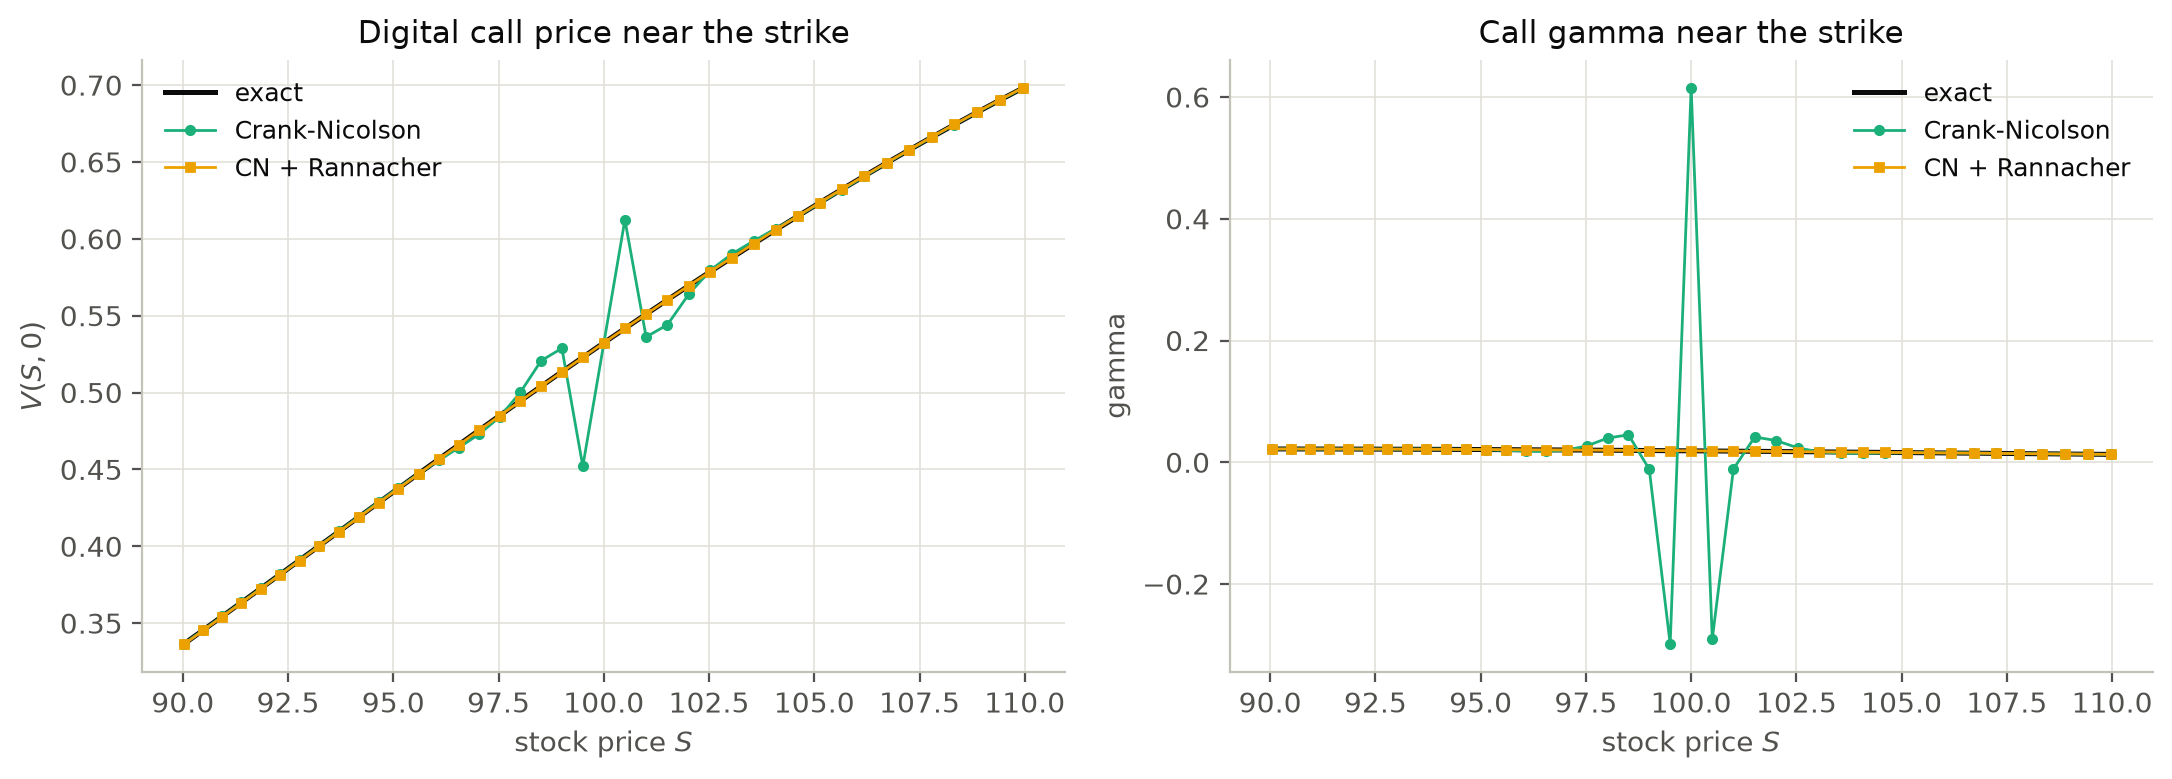
\includegraphics[width=\textwidth]{01_oscillations.png}
\caption{Crank-Nicolson with and without two Rannacher steps on a grid with $\lambda = 40$. The digital price (left) and the call gamma (right) oscillate near the strike without smoothing.}
\label{fig:osc}
\end{figure}

\subsection{Rannacher smoothing and the Greeks}

Rannacher smoothing is usually described with two implicit steps \citep{pooley2003}, and two are enough for the prices. Gamma is a harder test because it is a second derivative. Figure~\ref{fig:rannacher} repeats the convergence study for the gamma of the digital with 0, 2, 4 and 8 start-up steps. Without smoothing the error grows from 0.16 to 40 as the grid is refined. With two steps it stalls at about $10^{-4}$, around 14\% of the largest gamma, at the node next to the strike. With four or eight steps it falls at second order to below $3\times10^{-7}$. Two implicit steps damp the highest frequencies, but the jump also feeds slightly lower frequencies that two steps do not damp enough, and gamma is sensitive enough to see them. \citet{giles2006} analyse the start-up procedure in detail. Our practical conclusion is that the number of start-up steps should be chosen with the least smooth quantity required in mind, not just the price. Eight steps cost a little accuracy on coarse grids, since each implicit step adds an $O(\Delta\tau^2)$ local error, but they do not change the order.

\begin{figure}[htbp]
\centering
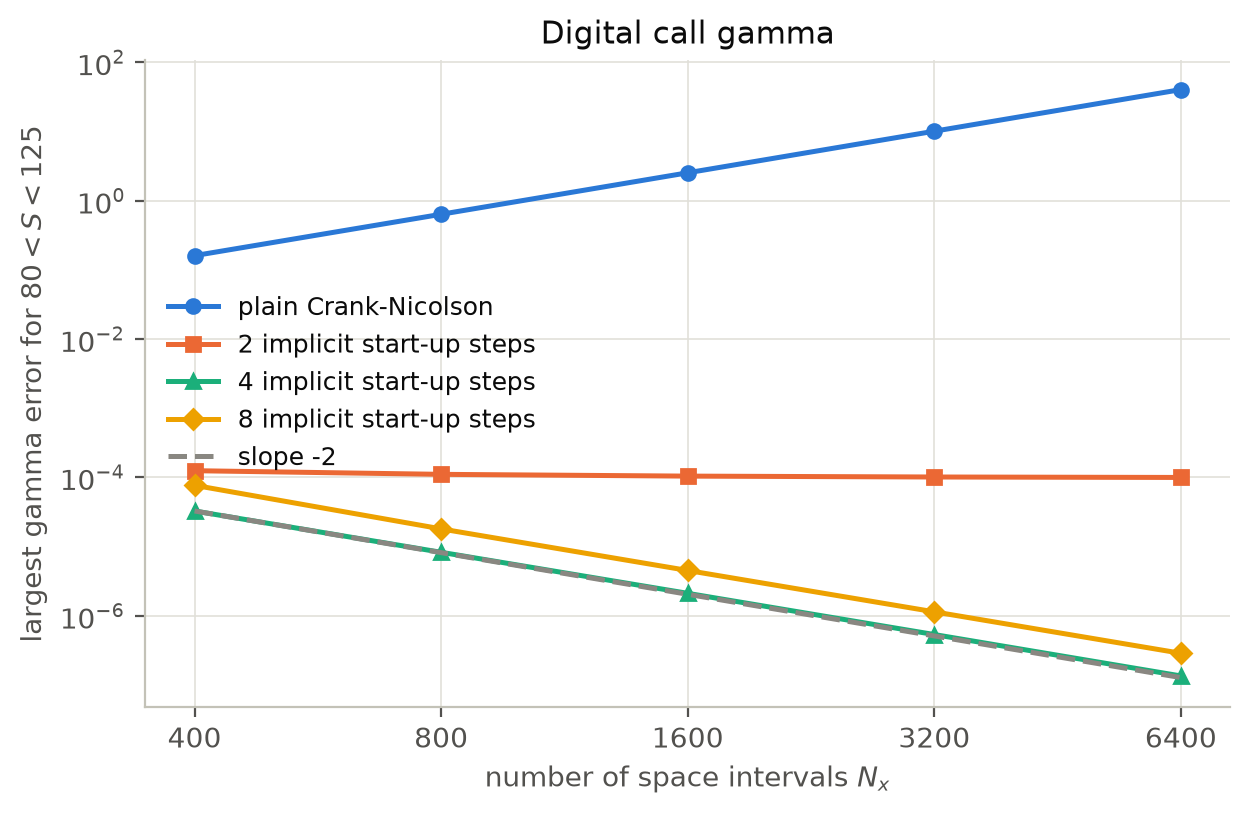
\includegraphics[width=0.62\textwidth]{01_rannacher_steps.png}
\caption{Largest error in the gamma of the digital over $80 < S < 125$ for different numbers of implicit start-up steps. Two steps leave an error that stops decreasing at about $10^{-4}$, while four restore second order convergence.}
\label{fig:rannacher}
\end{figure}

The Greeks also need care because the grid is uniform in $x$ rather than $S$. Central differences give $V_x$ and $V_{xx}$, and the chain rule with $\partial x/\partial S = 1/S$ gives
\begin{equation}
\Delta = \frac{V_x}{S}, \qquad \Gamma = \frac{V_{xx} - V_x}{S^2}. \label{eq:greeks}
\end{equation}
Using \eqref{eq:greeks}, the grid gamma of the call agrees with the closed form to $1.1\times10^{-6}$ and the grid delta to $8.4\times10^{-6}$. Omitting the $-V_x$ term gives an error of $7.5\times10^{-3}$, which is a modelling mistake rather than a discretisation error and does not shrink as the grid is refined.

\section{Monte Carlo simulation}\label{sec:mc}

\subsection{Exact sampling and Euler-Maruyama}

It\^o's formula applied to $\ln S$ gives the exact solution of \eqref{eq:gbm}, $S(T) = S_0\exp((r - \frac{1}{2}\sigma^2)T + \sigma\sqrt{T}z)$ with $z$ standard normal, so $S(T)$ can be sampled exactly in one step. For a model without a closed form solution we would instead use the Euler-Maruyama method of Notes~4.9,
\begin{equation}
S_{n+1} = S_n + rS_n\Delta t + \sigma S_n\Delta B_n, \qquad \Delta B_n = z_n\sqrt{\Delta t}. \label{eq:em}
\end{equation}
Our simulation advances both versions together, driven by the same increments $\Delta B_n$, applying the exact solution over each step for one and \eqref{eq:em} for the other. The difference between them at $T$ is then purely the Euler-Maruyama discretisation error, which is what makes its bias measurable in Section~\ref{sec:bias}.

\subsection{Statistical error}

With $M$ independent discounted payoffs the estimate is their sample mean, with standard error $s/\sqrt{M}$ (Notes~4.10), where $s = 14.71$ is the standard deviation of one discounted call payoff. Using exact sampling and repeating each experiment 50 times for $M$ from $10^2$ to $10^6$, the root mean square error over the repeats matches the single run standard error at every $M$, for example $1.50\times10^{-2}$ against $1.47\times10^{-2}$ at $M = 10^6$, and falls like $M^{-1/2}$. Of the 250 estimates, 237 (94.8\%) lie within $\pm1.96\,s/\sqrt{M}$ of the exact price. In a separate test the 95\% interval computed inside a single run with $M = 10^4$ contained the exact price in 382 of 400 runs (95.5\%). The standard error is therefore an honest error bar. The weakness of Monte Carlo is the rate itself, since each extra correct digit costs 100 times more paths, and even $10^7$ paths only give a 95\% interval of about $\pm0.01$.

\subsection{Time step bias and coupling}\label{sec:bias}

For an SDE scheme the strong error $\E|S_N - S(T)|$ measures the pathwise error and the weak error $|\E f(S_N) - \E f(S(T))|$ the error in an expectation, which is what a price is. Euler-Maruyama has strong order $\frac{1}{2}$ and weak order 1 \citep{higham2001}. The first order bias can be seen exactly in the mean. Each step of \eqref{eq:em} multiplies $S_n$ by an independent factor with mean $1 + r\Delta t$, so
\begin{equation}
\E[S_N] = S_0(1 + r\Delta t)^N = S_0e^{rT}\left(1 - \tfrac{1}{2}r^2T\Delta t + O(\Delta t^2)\right),
\end{equation}
a bias of $-\frac{1}{2}S_0e^{rT}r^2T\Delta t$, which agrees with the exact value to three significant figures for $N \ge 32$.

For the call price the bias is small, about $1.6\times10^{-3}$ at $N = 64$, while the standard error of an independent estimate with $10^6$ paths is about 0.015. Measured directly, the bias is buried in noise and even appears with the wrong sign at several step counts, and resolving it to 10\% would need around $10^{10}$ paths. With the coupled simulation we instead average the differences $e^{-rT}(f(S_N) - f(S(T)))$, which are of the size of the strong error and so have a small variance. Figure~\ref{fig:em} shows the result with $10^6$ paths. The bias falls from 0.25 with one step to $1.2\times10^{-3}$ with 128 steps, with a fitted weak order of 1.12, and the strong error falls from 2.05 to 0.21 with a fitted order of 0.47. The bias is negative, so Euler-Maruyama underprices the call, consistent with its underestimate of $\E[S(T)]$.

\begin{figure}[htbp]
\centering
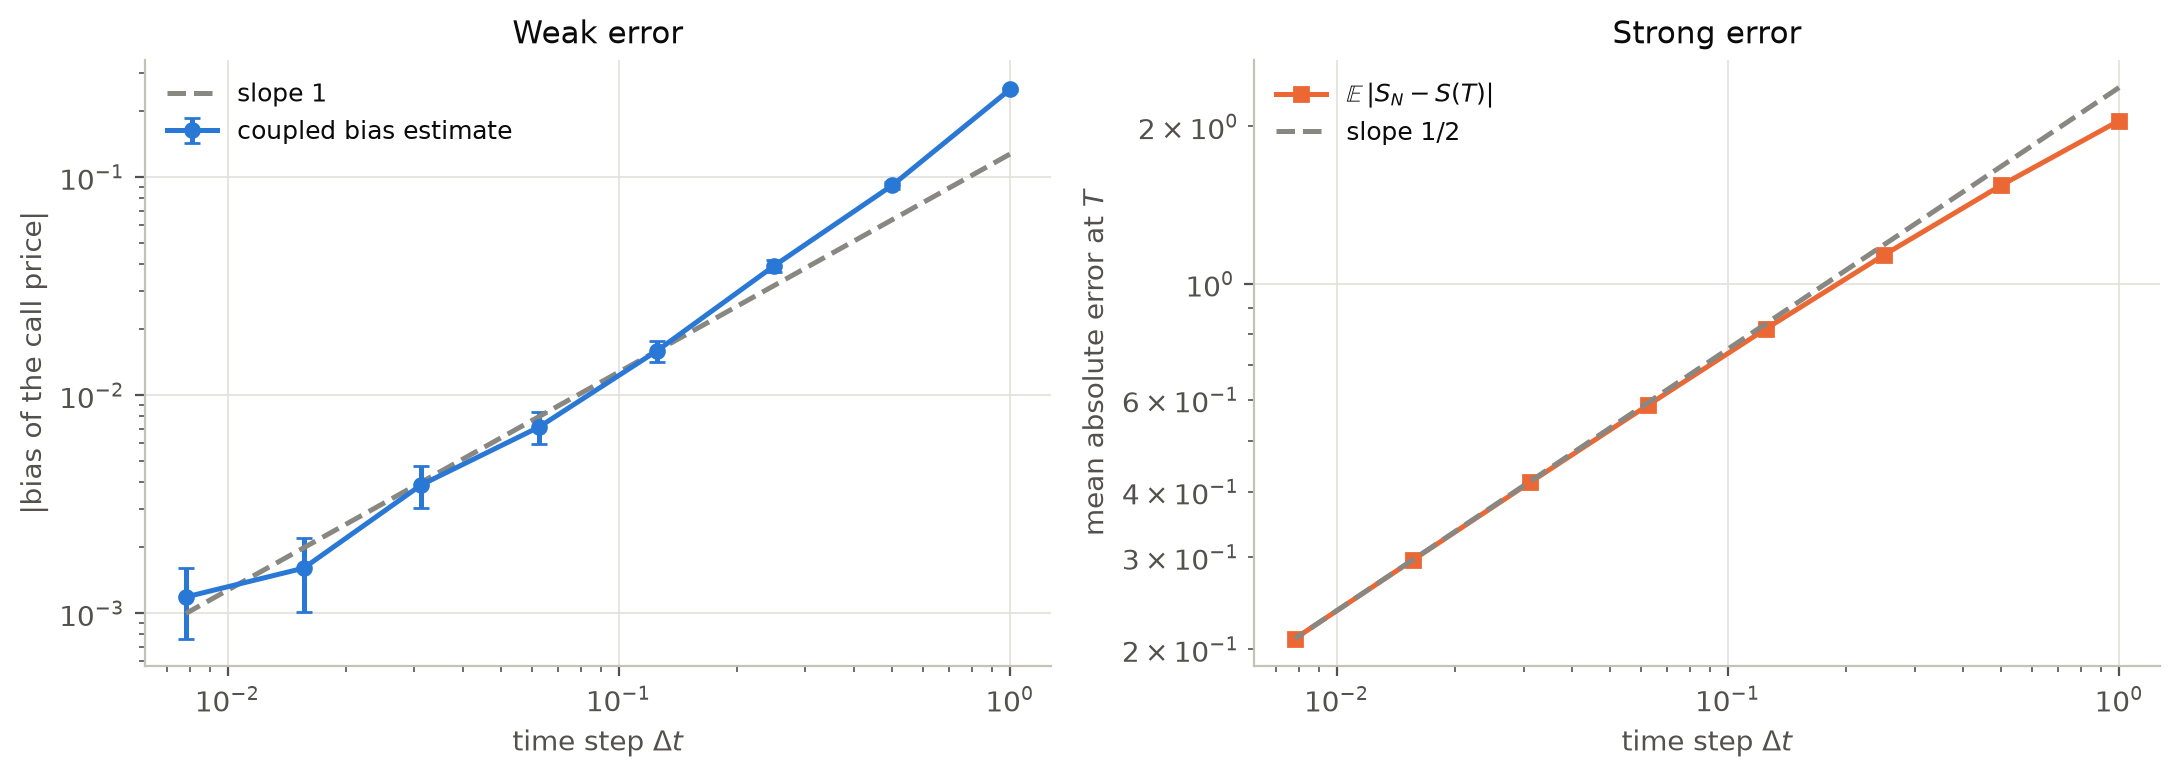
\includegraphics[width=\textwidth]{02_em_weak_strong.png}
\caption{Euler-Maruyama errors from $10^6$ coupled paths. The bias of the call price (left, with 95\% error bars) is first order in $\Delta t$, and the pathwise error at expiry (right) is of order one half.}
\label{fig:em}
\end{figure}

\subsection{Balancing bias and statistical error}

When both errors are present, a fixed budget must be divided between paths and time steps \citep{duffie1995}. With a bias of $c\Delta t$ and variance $s^2/M$, giving half of the mean square error to each term to reach a root mean square error $\varepsilon$ requires $N = \sqrt{2}\,cT/\varepsilon$ steps and $M = 2s^2/\varepsilon^2$ paths, a cost of $MN \propto \varepsilon^{-3}$, compared with $\varepsilon^{-2}$ for exact sampling. Table~\ref{tab:cost} evaluates this with our measured $c = 0.124$ and $s = 14.71$. For one cent accuracy the time stepped simulation needs 36 times as many random numbers as exact sampling, and the factor grows like $1/\varepsilon$. For geometric Brownian motion this simply says never to time step, but for models without an exact solution the $\varepsilon^{-3}$ cost of a first order scheme is unavoidable, and reducing it is the purpose of the multilevel method of \citet{giles2008}.

\begin{table}[htbp]
\centering
\caption{Work needed to reach a root mean square error $\varepsilon$ with Euler-Maruyama and with exact sampling, using the measured bias constant and payoff standard deviation.}
\label{tab:cost}
\begin{tabular}{cccccc}
\toprule
$\varepsilon$ & EM steps & EM paths & EM normals drawn & Exact paths & Ratio \\
\midrule
$10^{-1}$ & 2 & $4.3\times10^{4}$ & $8.7\times10^{4}$ & $2.2\times10^{4}$ & 4 \\
$10^{-2}$ & 18 & $4.3\times10^{6}$ & $7.8\times10^{7}$ & $2.2\times10^{6}$ & 36 \\
$10^{-3}$ & 176 & $4.3\times10^{8}$ & $7.6\times10^{10}$ & $2.2\times10^{8}$ & 352 \\
\bottomrule
\end{tabular}
\end{table}

\section{Grids against Monte Carlo as the dimension grows}\label{sec:dim}

\subsection{One dimension}

In one dimension the comparison is one sided. The Crank-Nicolson solver with Rannacher smoothing and $N_\tau = N_x/10$ reaches an error of $2.7\times10^{-6}$ at $S_0$ in 0.37 seconds, with its error falling like the inverse of the work $N_xN_\tau$ (fitted slope $-1.00$). Exact sampling Monte Carlo has a standard error of $4.7\times10^{-3}$ after 0.42 seconds with $10^7$ paths, and would need about $3\times10^{13}$ paths, around two weeks of computing, to match the PDE.

\subsection{Convergence exponents}

Suppose a grid method has error $O(h^p)$ with $n$ points per axis. A tensor product grid in $d$ dimensions has $W = n^d$ points, so
\begin{equation}
\varepsilon \propto n^{-p} = W^{-p/d}, \label{eq:gridrate}
\end{equation}
while Monte Carlo has $\varepsilon \propto W^{-1/2}$ in every dimension \citep[Section 1.1]{glasserman2004}. For second order quadrature the grid exponent $-2/d$ is steeper than $-\frac{1}{2}$ for $d < 4$ and shallower for $d > 4$. A PDE solver also steps in time. With Crank-Nicolson and $\Delta\tau \propto \Delta x$ the work is $W = n^{d+1}$ and $\varepsilon \propto W^{-2/(d+1)}$, which loses to Monte Carlo beyond $d = 3$. For the explicit scheme the stability condition forces $\Delta\tau \propto \Delta x^2$, so $W = n^{d+2}$, $\varepsilon \propto W^{-2/(d+2)}$, and the crossover falls to $d = 2$. In this sense the stability analysis of Section~\ref{sec:pde} costs the explicit scheme a whole dimension. These exponents only describe the limit of small $\varepsilon$, and the constants decide the crossover at a practical accuracy.

The Monte Carlo rate does not depend on the dimension, but its constant can. The hit or miss estimate of the volume of the unit ball (exercise R4.2) samples the cube $[-1,1]^d$ and has relative standard error $\sqrt{(1-p)/(pM)}$, where $p = V_d/2^d$ is the fraction of the cube inside the ball. As Figure~\ref{fig:ball} shows, $p$ falls to $3.3\times10^{-4}$ at $d = 12$, and the relative error with $10^6$ points grows a hundredfold between $d = 2$ and $d = 12$, exactly as predicted. The same issue arises in pricing whenever the payoff is a rare event, such as a deep out of the money option, and the remedy is to sample more cleverly, for example by importance sampling.

\begin{figure}[htbp]
\centering
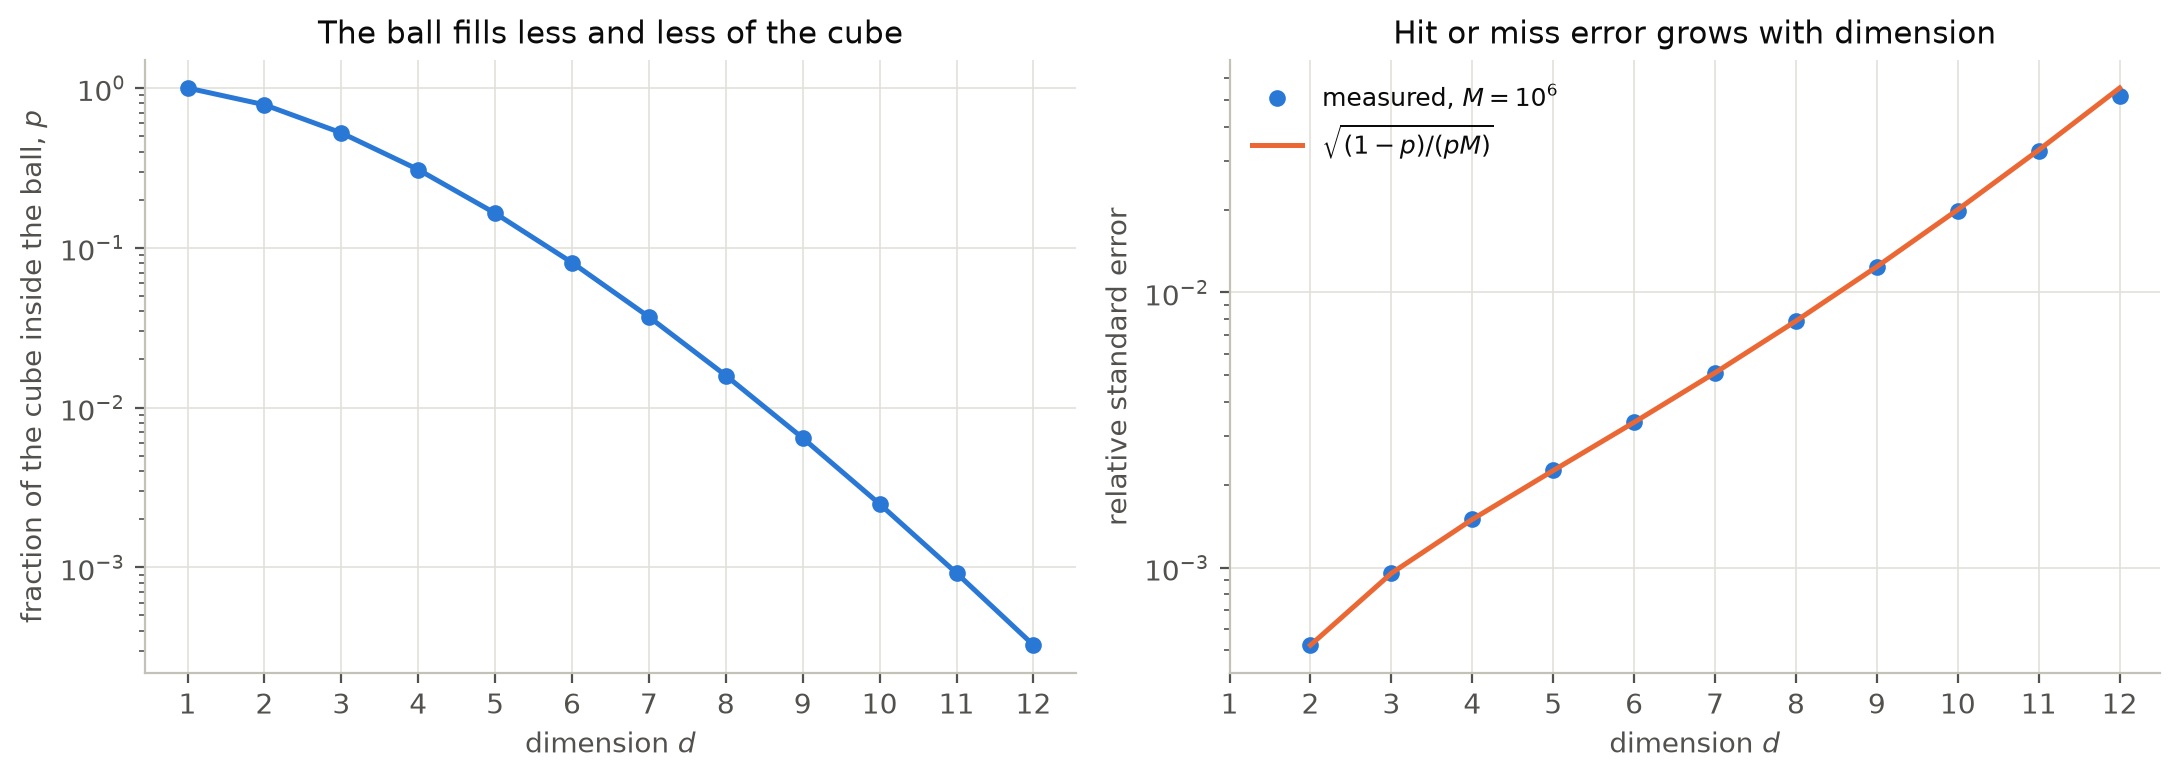
\includegraphics[width=\textwidth]{03_ball_volume.png}
\caption{Hit or miss Monte Carlo for the volume of the unit ball. The fraction of the cube inside the ball collapses with dimension (left), so the relative error with $10^6$ points grows as $\sqrt{(1-p)/(pM)}$ predicts (right).}
\label{fig:ball}
\end{figure}

\subsection{A pricing problem in \texorpdfstring{$d$}{d} dimensions}

To measure the crossover we need a $d$ dimensional pricing problem with an exact answer. We use a call on the geometric average of $d$ independent stocks with the same parameters as before. With $z_1, \dots, z_d$ the standard normals driving the stocks,
\begin{equation}
G(T) = S_0\exp\left(\left(r - \tfrac{1}{2}\sigma^2\right)T + \sigma\sqrt{T}\,\frac{z_1 + \dots + z_d}{d}\right), \qquad V = e^{-rT}\,\E\max(G(T) - K, 0),
\end{equation}
and since $\ln G(T)$ is normal, $V$ has a closed form of Black-Scholes type, given in Section~\ref{sec:basket}. The grid method is the tensor product trapezoid rule with $n$ points per axis on $[-6, 6]$, the quadrature analogue of a PDE grid without time stepping, and Monte Carlo samples the $z_i$ directly. The integrand depends only on $z_1 + \dots + z_d$, so the problem could be reduced to one dimension by symmetry (Notes~4.2.1). We deliberately do not do this, because the geometric basket stands in for products such as the arithmetic basket, where no such reduction exists.

\begin{figure}[htbp]
\centering
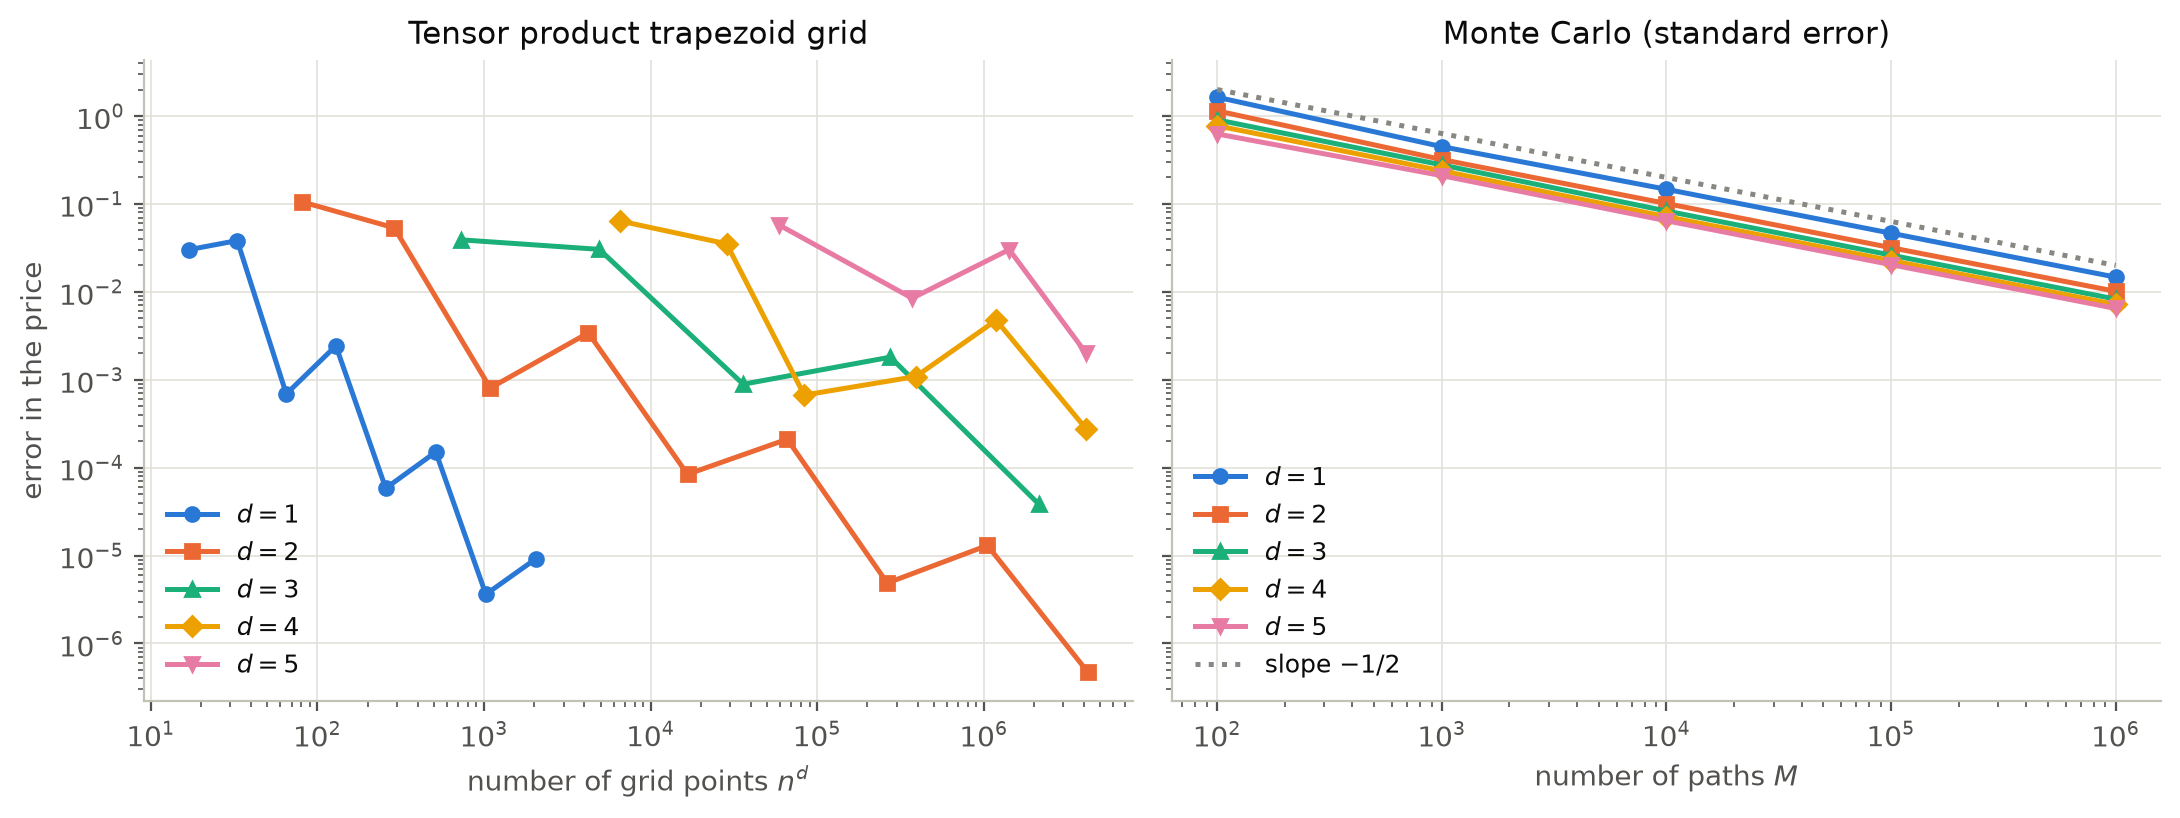
\includegraphics[width=\textwidth]{03_grid_vs_mc_by_dimension.png}
\caption{Error in the geometric basket price against the number of function evaluations for $d = 1$ to 5. The grid curves flatten and shift right as $d$ grows, while every Monte Carlo curve has slope $-\frac{1}{2}$.}
\label{fig:gridmc}
\end{figure}

Figure~\ref{fig:gridmc} shows the measured errors for $d = 1$ to 5. The Monte Carlo lines all have slope $-\frac{1}{2}$ and lie close together. They move slightly down as $d$ grows because the average of $d$ independent stocks has volatility $\sigma/\sqrt{d}$, so the payoff standard deviation falls from 14.7 at $d = 1$ to 6.5 at $d = 5$. The grid lines flatten and move right as $d$ increases, with fitted slopes of $-1.93$, $-1.07$, $-0.84$, $-0.72$ and $-0.61$. These are close to $-2/d$ for $d \le 2$ and steeper than it for $d \ge 3$, where memory limits us to coarse, pre-asymptotic grids. The grid errors also jump by a factor of about 4 between neighbouring grids. The kink of the payoff lies on the plane where $z_1 + \dots + z_d$ is constant, and the trapezoid error depends on where that plane falls relative to the grid points, as in exercise R1.3.

\begin{figure}[htbp]
\centering
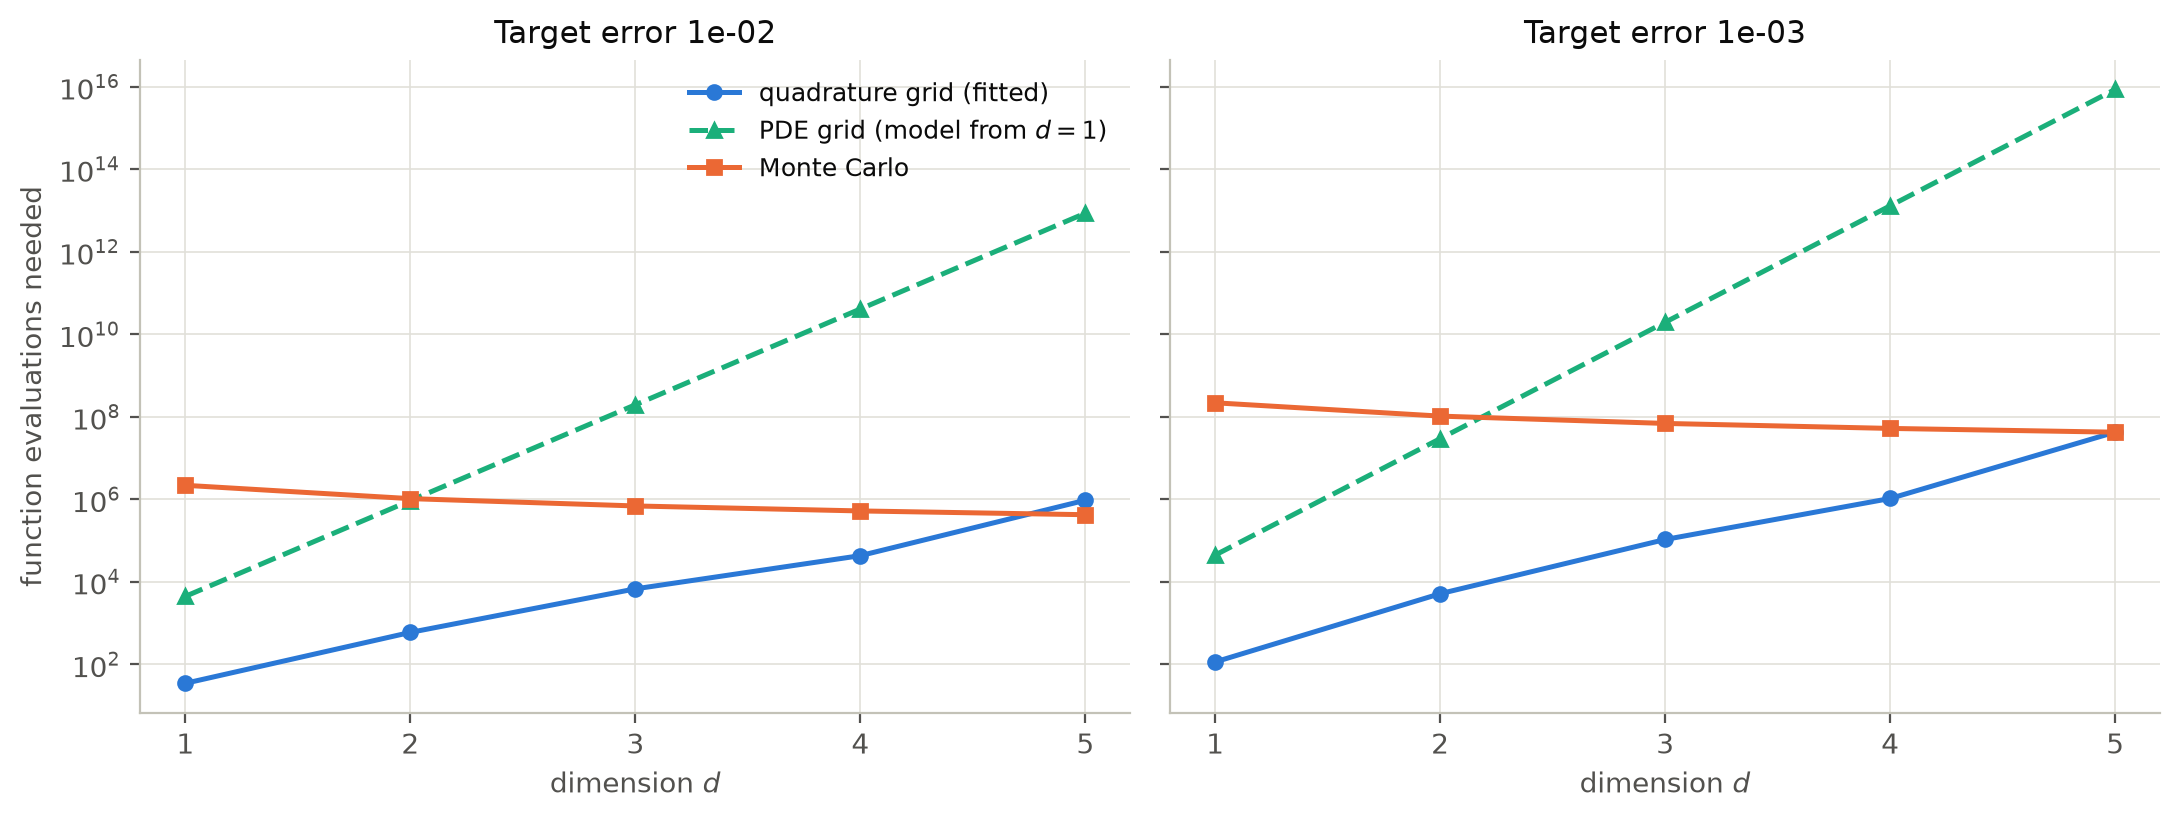
\includegraphics[width=\textwidth]{03_crossover.png}
\caption{Function evaluations needed to reach a target error of $10^{-2}$ (left) and $10^{-3}$ (right), from the fitted grid convergence, the measured Monte Carlo variance, and a model of a time stepping PDE solver extrapolated from one dimension.}
\label{fig:crossover}
\end{figure}

Inverting the fitted lines gives the number of evaluations each method needs to reach a target error, shown in Figure~\ref{fig:crossover}. For Monte Carlo it is $(s_d/\varepsilon)^2$, with $s_d$ the payoff standard deviation. We also include a model of a $d$ dimensional Crank-Nicolson solver that needs the same resolution per axis as our one dimensional solver, whose error was $440/N_x^2$, so that $W = N_x^{d+1}/10$. This curve is an extrapolation from $d = 1$ rather than a measurement. At $\varepsilon = 10^{-2}$ quadrature needs fewer evaluations than Monte Carlo up to $d = 4$, with $4.3\times10^4$ against $5.2\times10^5$, but more at $d = 5$, with $9.4\times10^5$ against $4.2\times10^5$. At $\varepsilon = 10^{-3}$ the two are level at $d = 5$. This is a little later than the asymptotic prediction of $d = 4$, mainly because the coarse grids converge faster than their asymptotic rate, partly offset by the falling payoff variance that helps Monte Carlo. The PDE model is level with Monte Carlo at $d = 2$ and loses clearly from $d = 3$, where it needs about $2\times10^8$ evaluations against $7\times10^5$, as the exponent $-2/(d+1)$ predicts.

\section{Extension to basket options on correlated stocks}\label{sec:basket}

With 20 correlated stocks a grid with only 10 points per axis would need $10^{20}$ points, so Monte Carlo is the only practical method. Each stock follows its own geometric Brownian motion, $S_i(T) = S_{0,i}\exp((r - \frac{1}{2}\sigma_i^2)T + \sigma_iW_i(T))$, with $\mathrm{corr}(W_i, W_j) = C_{ij}$. We take $S_{0,i} = 100$, $\sigma_i = 0.2$ and equal pairwise correlation $\rho$, so $C = (1-\rho)I + \rho\mathbf{1}\mathbf{1}^T$. Its eigenvalues are $1 + (d-1)\rho$ and $1 - \rho$, so it is positive definite exactly when $-1/(d-1) < \rho < 1$. Correlated normals are generated with the Cholesky factorisation $C = LL^T$ \citep[Section 2.6]{sauer2018}, since if $z$ has covariance $I$ then $Lz$ has covariance $LL^T = C$.

The arithmetic basket call, with payoff $\max(A - K, 0)$ where $A = \frac{1}{d}\sum_iS_i(T)$, has no closed form. The geometric average $G$ satisfies $\ln G = \frac{1}{d}\sum_i\ln S_i(T)$, which is normal with mean $\mu = \frac{1}{d}\sum_i(\ln S_{0,i} + (r - \frac{1}{2}\sigma_i^2)T)$ and variance $v = \frac{T}{d^2}\sum_{i,j}\sigma_i\sigma_jC_{ij}$, so
\begin{equation}
V_G = e^{-rT}\left(e^{\mu + v/2}N(d_1) - KN(d_2)\right), \qquad d_2 = \frac{\mu - \ln K}{\sqrt{v}}, \quad d_1 = d_2 + \sqrt{v}. \label{eq:geo}
\end{equation}
We use \eqref{eq:geo} twice. First it verifies the correlated simulation. In 12 comparisons with $d \in \{2, 5, 10, 20\}$ and $\rho \in \{0, 0.3, 0.7\}$, eleven Monte Carlo prices lie within two standard errors of \eqref{eq:geo}. The twelfth, with $\rho = 0.7$ and $d = 10$, is at $z = 2.65$, an outcome that happens by chance in about 9\% of sets of 12 comparisons. Ten fresh runs of that case gave $z$ between $-2.0$ and $2.5$ with mean $-0.20$, well within the $\pm0.63$ expected, so it was a fluctuation rather than a bias.

Second, the geometric payoff is a control variate. With $Y$ and $X$ the discounted arithmetic and geometric payoffs, $Y_{\mathrm{cv}} = Y - b(X - \E X)$ has the same mean as $Y$ for any $b$, and the choice $b = \mathrm{Cov}(X,Y)/\mathrm{Var}(X)$ gives
\begin{equation}
\mathrm{Var}(Y_{\mathrm{cv}}) = (1 - \rho_{XY}^2)\,\mathrm{Var}(Y),
\end{equation}
where $\rho_{XY}$ is the correlation between the two payoffs \citep{kemna1990}. Since $A \ge G$ on every path and the two move almost together, $\rho_{XY}$ is very close to 1. Figure~\ref{fig:cv} shows variance reduction factors from 70 down to 25 for independent stocks, about 160 to 210 for $\rho = 0.3$, and 1250 to 2290 for $\rho = 0.7$, with $\rho_{XY}$ between 0.980 and 0.9998. For 20 stocks with $\rho = 0.3$ the control variate gives $7.3567 \pm 0.0026$ from 200000 paths, against $7.340 \pm 0.039$ for plain Monte Carlo (95\% intervals), which would need about 211 times as many paths to match. A Taylor expansion gives $A/G \approx 1 + \frac{1}{2}\eta^2$, where $\eta^2$ is the variance of the log prices across the basket, and this explains the trends. Correlated stocks stay close together, so the two payoffs nearly coincide. For independent stocks the average becomes less volatile as $d$ grows but the spread between stocks does not, so more of the remaining variance is invisible to the control variate. The cost per path grew roughly linearly in $d$, and $10^5$ paths with $d = 100$ took about half a second.

\begin{figure}[htbp]
\centering
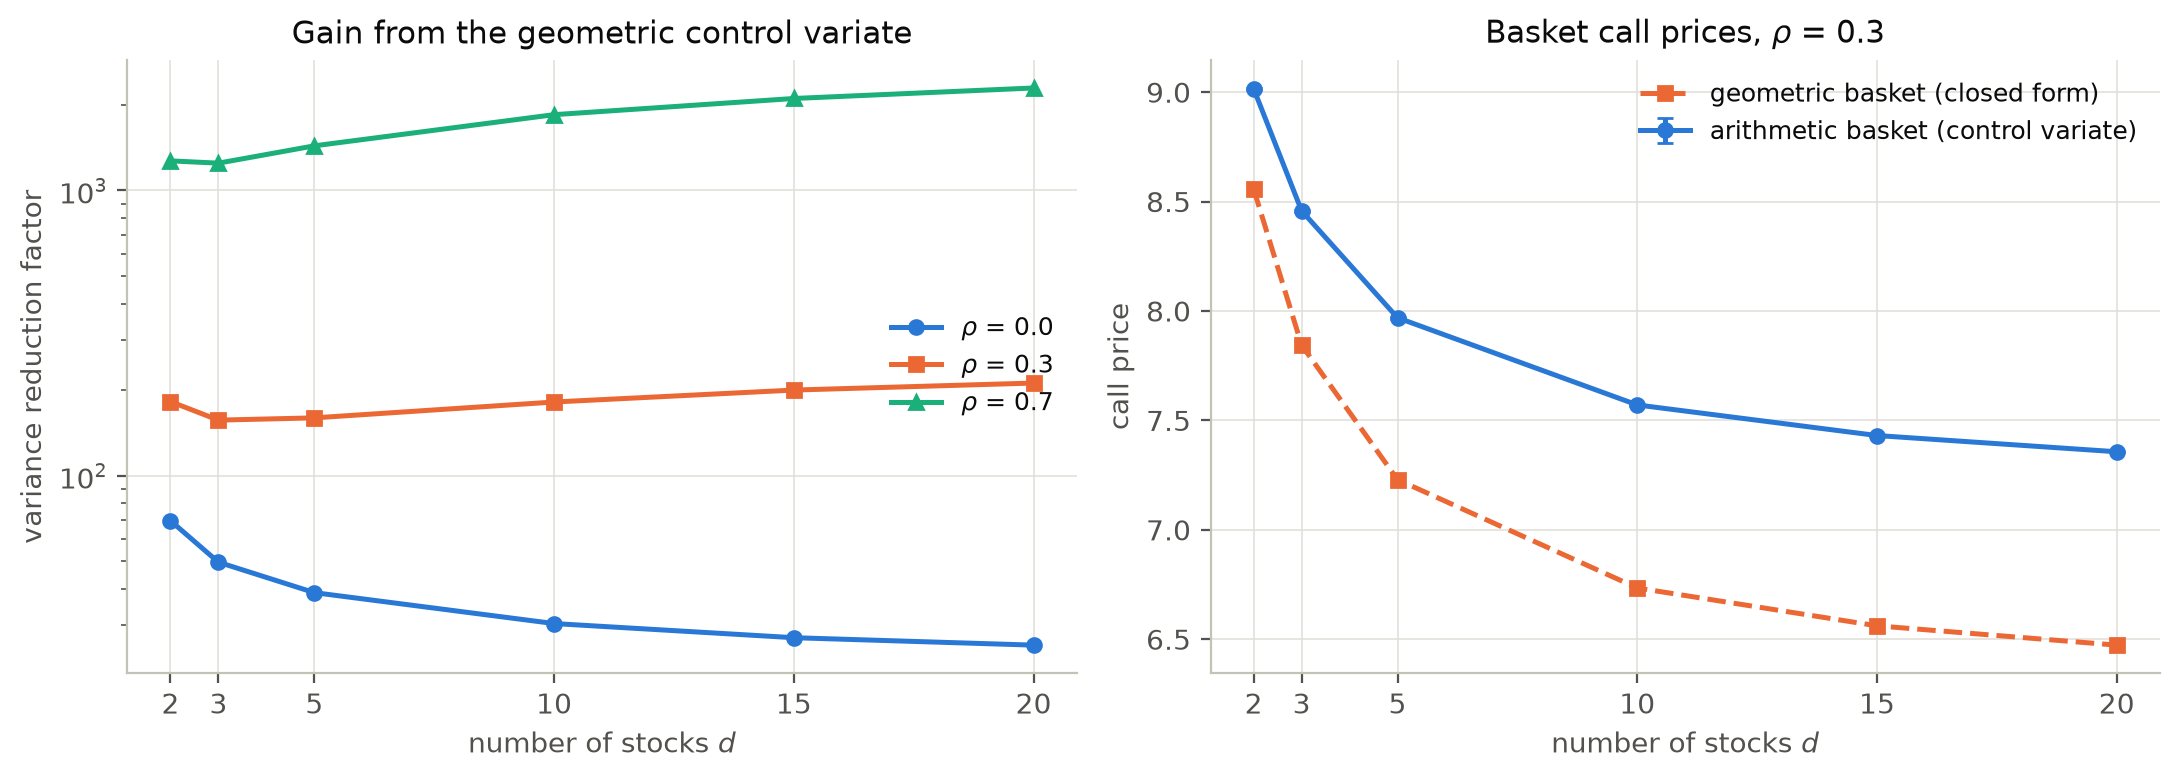
\includegraphics[width=\textwidth]{04_control_variate.png}
\caption{Variance reduction from the geometric basket control variate (left), and the arithmetic basket price with its control variate estimate against the geometric closed form for $\rho = 0.3$ (right).}
\label{fig:cv}
\end{figure}

\section{Verification and validation}\label{sec:vv}

\citet{babuska2004} separate two questions that are easy to confuse. Verification asks whether a program solves its mathematical model accurately, which they summarise as solving the equations right. Validation asks whether the model describes the real system accurately enough, or solving the right equations. This project puts most of its effort into verification, at three levels. First, every method is compared with an exact closed form price, and an automated test suite in the repository repeats these checks. Second, we check convergence rates rather than single numbers. The observed orders of second order for Crank-Nicolson with Rannacher smoothing, first order for the implicit scheme, weak order one and strong order one half for Euler-Maruyama, and $M^{-1/2}$ for Monte Carlo all match the theory. This is a much stronger test than matching one number, because most bugs change the order of convergence even when they leave the answer roughly right. Third, we check the error estimates themselves, through the 95.5\% coverage of the Monte Carlo intervals and the re-testing of the one outlying comparison in Section~\ref{sec:basket}. For the arithmetic basket, which has no exact price, the geometric benchmark verifies the simulation, and the plain and control variate estimates agree to within about 1.2 standard errors in all 18 cases.

Validation is a different matter, and we have not done it. The Black-Scholes model assumes a constant volatility, normally distributed log returns, continuous trading and no transaction costs, and none of these hold exactly. In real markets the volatility implied by observed option prices depends on the strike, and stock returns have heavier tails than the normal distribution allows. The prices computed here are therefore exact prices for the Black-Scholes model, not predictions of market prices. The conclusions about numerical methods should still carry over to more realistic models, which mostly make them more pressing. The stochastic volatility model of \citet{heston1993} adds a second state variable, so its PDE is two dimensional, and a volatility depending on $S$ and $t$ removes the exact solution of the SDE, so the time stepping bias of Section~\ref{sec:mc} can no longer be avoided.

\section{Discussion}\label{sec:discussion}

Option prices are quoted in cents, so a natural accuracy target for our call, worth about 10.45, is $10^{-2}$, about 0.1\%. The Crank-Nicolson solver with Rannacher smoothing reaches this with a couple of hundred grid points in about a millisecond, while plain Monte Carlo needs around two million paths to bring its standard error down to one cent, roughly a hundred times longer. Risk systems revalue whole portfolios under many market scenarios every day, so differences in speed of this size decide which methods are practical. The Greeks matter as much as the price. Delta is the number of shares held to hedge each option and gamma measures how quickly that hedge must be adjusted, so the plain Crank-Nicolson gamma of Section~\ref{sec:pde}, wrong by 0.6 against a true value of about 0.02, would make a hedger trade far too much near the strike. This is why the oscillation problem matters even when the price looks fine. Our crossover also agrees with how the work is usually divided in practice. Problems with one or two underlying variables are normally solved with PDE methods or trees, while baskets and path dependent products are normally priced by Monte Carlo, and our measurements give a quantitative reason for that split.

The study has several limitations. All the options are European with constant volatility and interest rate, chosen so that exact answers exist, which is also the setting where numerical methods are needed least. The PDE grid is uniform, while practical codes concentrate points near the strike. The geometric basket is unusually kind to both methods, since its payoff variance falls with $d$ and its integrand secretly depends on a single combination of the variables. The crossover curve for a $d$ dimensional PDE is a model extrapolated from one dimension rather than a measurement, and the fitted grid rates for $d \ge 3$ are pre-asymptotic. Better methods exist on both sides. Sparse grids and alternating direction implicit schemes push the grid crossover upwards, while quasi-Monte Carlo and further variance reduction push it down. The natural next steps are products without closed forms, such as American options, which turn the PDE into a free boundary problem, and local volatility models, which break the heat equation transform and make time stepping unavoidable.

\section{Conclusions}\label{sec:conclusions}

The Feynman-Kac formula gives two routes to the same price, and on problems with exact answers we measured how each behaves. On the PDE side the heat equation transform makes the explicit stability limit independent of the grid extent, and Crank-Nicolson with practical time steps fails near a non-smooth payoff, losing an order for the call and failing to converge at all for the digital. Rannacher smoothing restores second order convergence, but the gamma of the digital needs four implicit start-up steps rather than the usual two. On the Monte Carlo side the statistical error and the Euler-Maruyama bias behave exactly as theory predicts once they are separated by coupling, and together they raise the cost from $\varepsilon^{-2}$ to $\varepsilon^{-3}$. Comparing the two, a second order grid is better by many orders of magnitude in one dimension, but its convergence rate per unit of work decays like $2/d$, or $2/(d+1)$ with time stepping, while Monte Carlo keeps $\frac{1}{2}$. The measured crossover is at about four to five dimensions for quadrature and about three for a time stepping PDE solver, and beyond it Monte Carlo, helped by a good control variate, prices a 20 stock basket accurately in a fraction of a second.

\section{Self-assessment}\label{sec:self}

The project sheet invites an optional self-assessment. The grade claimed for this project is a 7, justified below against the four criteria used to award additional points.

For knowledge and content mastery, the project derives rather than quotes its main results, including the transformation of the Black-Scholes equation into the heat equation, the von Neumann stability analysis of the explicit and Crank-Nicolson schemes, the first order bias of Euler-Maruyama in the mean, the variance of the control variate estimator and the convergence exponents that decide the crossover dimension. It uses material from every module of the course, from finite differences and discontinuities in Module 1 to banded systems and the Cholesky factorisation in Module 2, time stepping and stiffness in Module 3, and PDEs, Monte Carlo methods, SDEs and error estimation in Module 4.

For critical evaluation and insight, several results came from refusing to take a first answer at face value. Measuring the error over a window of stock prices, rather than only at the strike, exposed a Crank-Nicolson failure that the usual single point check hides. Coupling the exact and approximate paths made an Euler-Maruyama bias measurable when it would otherwise have been lost in the noise. An outlying comparison in Section~\ref{sec:basket} was tested with fresh simulations rather than ignored or explained away. The limitations of each experiment are stated where they arise, including the pre-asymptotic grid fits, the unusually kind test problem and the absence of validation against market data.

For originality, the project goes beyond reproducing textbook results. It finds that the usual two Rannacher steps are not enough for the gamma of a digital option while four are, it shows that the explicit scheme's stability limit costs a whole dimension in the crossover, and it measures the crossover directly on a problem with an exact answer in every dimension. The extension prices a 20 stock basket with a variance reduction factor of over 2000.

For communication, every result is presented with a figure or table and a short explanation tied back to the course notes, the derivations are written out in full, and the code is short, commented and backed by automated tests, with fixed random seeds so that every number in this report can be reproduced from the public repository.

\begin{thebibliography}{24}

\bibitem[Babu\v{s}ka and Oden(2004)]{babuska2004}
Babu\v{s}ka, I. and Oden, J. T. (2004). Verification and validation in computational engineering and science: basic concepts. \emph{Computer Methods in Applied Mechanics and Engineering}, 193, 4057-4066.

\bibitem[Bellman(1957)]{bellman1957}
Bellman, R. (1957). \emph{Dynamic Programming}. Princeton University Press.

\bibitem[Black and Scholes(1973)]{black1973}
Black, F. and Scholes, M. (1973). The pricing of options and corporate liabilities. \emph{Journal of Political Economy}, 81(3), 637-654.

\bibitem[Boyle(1977)]{boyle1977}
Boyle, P. P. (1977). Options: a Monte Carlo approach. \emph{Journal of Financial Economics}, 4(3), 323-338.

\bibitem[Brennan and Schwartz(1978)]{brennan1978}
Brennan, M. J. and Schwartz, E. S. (1978). Finite difference methods and jump processes arising in the pricing of contingent claims: a synthesis. \emph{Journal of Financial and Quantitative Analysis}, 13(3), 461-474.

\bibitem[Bungartz and Griebel(2004)]{bungartz2004}
Bungartz, H.-J. and Griebel, M. (2004). Sparse grids. \emph{Acta Numerica}, 13, 147-269.

\bibitem[Crank and Nicolson(1947)]{crank1947}
Crank, J. and Nicolson, P. (1947). A practical method for numerical evaluation of solutions of partial differential equations of the heat-conduction type. \emph{Mathematical Proceedings of the Cambridge Philosophical Society}, 43(1), 50-67.

\bibitem[Duffie and Glynn(1995)]{duffie1995}
Duffie, D. and Glynn, P. (1995). Efficient Monte Carlo simulation of security prices. \emph{The Annals of Applied Probability}, 5(4), 897-905.

\bibitem[Feynman(1948)]{feynman1948}
Feynman, R. P. (1948). Space-time approach to non-relativistic quantum mechanics. \emph{Reviews of Modern Physics}, 20(2), 367-387.

\bibitem[Giles(2008)]{giles2008}
Giles, M. B. (2008). Multilevel Monte Carlo path simulation. \emph{Operations Research}, 56(3), 607-617.

\bibitem[Giles and Carter(2006)]{giles2006}
Giles, M. B. and Carter, R. (2006). Convergence analysis of Crank-Nicolson and Rannacher time-marching. \emph{Journal of Computational Finance}, 9(4), 89-112.

\bibitem[Glasserman(2004)]{glasserman2004}
Glasserman, P. (2004). \emph{Monte Carlo Methods in Financial Engineering}. Springer, New York.

\bibitem[Heston(1993)]{heston1993}
Heston, S. L. (1993). A closed-form solution for options with stochastic volatility with applications to bond and currency options. \emph{The Review of Financial Studies}, 6(2), 327-343.

\bibitem[Higham(2001)]{higham2001}
Higham, D. J. (2001). An algorithmic introduction to numerical simulation of stochastic differential equations. \emph{SIAM Review}, 43(3), 525-546.

\bibitem[Kac(1949)]{kac1949}
Kac, M. (1949). On distributions of certain Wiener functionals. \emph{Transactions of the American Mathematical Society}, 65(1), 1-13.

\bibitem[Kemna and Vorst(1990)]{kemna1990}
Kemna, A. G. Z. and Vorst, A. C. F. (1990). A pricing method for options based on average asset values. \emph{Journal of Banking and Finance}, 14(1), 113-129.

\bibitem[Maruyama(1955)]{maruyama1955}
Maruyama, G. (1955). Continuous Markov processes and stochastic equations. \emph{Rendiconti del Circolo Matematico di Palermo}, 4(1), 48-90.

\bibitem[Merton(1973)]{merton1973}
Merton, R. C. (1973). Theory of rational option pricing. \emph{The Bell Journal of Economics and Management Science}, 4(1), 141-183.

\bibitem[Metropolis and Ulam(1949)]{metropolis1949}
Metropolis, N. and Ulam, S. (1949). The Monte Carlo method. \emph{Journal of the American Statistical Association}, 44(247), 335-341.

\bibitem[Nieminen and Stilgoe(2026)]{notes2026}
Nieminen, T. and Stilgoe, A. (2026). \emph{COSC2500/COSC7500 Numerical Methods in Computational Science}, course notes. School of Mathematics and Physics, The University of Queensland.

\bibitem[Pooley et~al.(2003)]{pooley2003}
Pooley, D. M., Vetzal, K. R. and Forsyth, P. A. (2003). Convergence remedies for non-smooth payoffs in option pricing. \emph{Journal of Computational Finance}, 6(4), 25-40.

\bibitem[Rannacher(1984)]{rannacher1984}
Rannacher, R. (1984). Finite element solution of diffusion problems with irregular data. \emph{Numerische Mathematik}, 43(2), 309-327.

\bibitem[Sauer(2018)]{sauer2018}
Sauer, T. (2018). \emph{Numerical Analysis}, 3rd edition. Pearson.

\bibitem[Wilmott et~al.(1995)]{wilmott1995}
Wilmott, P., Howison, S. and Dewynne, J. (1995). \emph{The Mathematics of Financial Derivatives: A Student Introduction}. Cambridge University Press.

\end{thebibliography}

\appendix

\section{Code excerpts}\label{app:code}

The full code is in the \texttt{pricing} folder of the repository. The three excerpts below carry the main ideas of Sections~\ref{sec:pde}, \ref{sec:mc} and~\ref{sec:basket}.

The time stepping loop of the theta scheme \eqref{eq:theta}, from \texttt{pde.py}. The first \texttt{n\_rannacher} steps use $\theta = 1$, and the tridiagonal system is stored by diagonals for the banded solver.

\begin{lstlisting}
for n in range(n_steps):
    th = 1.0 if n < n_rannacher else theta

    # Right hand side from the known time level n:
    # (1 - 2(1 - theta) lam) u_j + (1 - theta) lam (u_{j-1} + u_{j+1})
    rhs = (1 - 2 * (1 - th) * lam) * u[1:-1] + (1 - th) * lam * (u[:-2] + u[2:])

    u_new = np.empty_like(u)
    u_new[0] = left[n + 1]
    u_new[-1] = right[n + 1]

    if th == 0:
        # Explicit Euler: nothing to solve.
        u_new[1:-1] = rhs
    else:
        # Implicit part: (1 + 2 theta lam) u_j - theta lam (u_{j-1} + u_{j+1}) = rhs.
        # The known boundary values at level n + 1 move to the right hand side.
        rhs[0] += th * lam * u_new[0]
        rhs[-1] += th * lam * u_new[-1]

        # Tridiagonal matrix stored by diagonals for scipy's banded solver:
        # row 0 is the super diagonal, row 1 the main diagonal, row 2 the sub diagonal.
        ab = np.zeros((3, m))
        ab[0, 1:] = -th * lam
        ab[1, :] = 1 + 2 * th * lam
        ab[2, :-1] = -th * lam
        u_new[1:-1] = solve_banded((1, 1), ab, rhs)

    u = u_new
\end{lstlisting}

The coupled simulation of Section~\ref{sec:bias}, from \texttt{sde.py}. The exact solution and the Euler-Maruyama approximation share every Brownian increment.

\begin{lstlisting}
dt = T / n_steps
S_exact = np.full(n_paths, float(S0))
S_em = np.full(n_paths, float(S0))

for n in range(n_steps):
    dB = np.sqrt(dt) * rng.standard_normal(n_paths)
    # Euler-Maruyama step
    S_em = S_em + r * S_em * dt + sigma * S_em * dB
    # Exact step: the solution formula applied over one interval of length dt
    S_exact = S_exact * np.exp((r - 0.5 * sigma**2) * dt + sigma * dB)
\end{lstlisting}

The correlated simulation and the control variate estimate of Section~\ref{sec:basket}, from \texttt{basket.py}.

\begin{lstlisting}
L = np.linalg.cholesky(corr)
z = rng.standard_normal((n_paths, d))
# Each row of z @ L.T is L times a row of z, so it has covariance C.
W = np.sqrt(T) * (z @ L.T)
S_T = S0 * np.exp((r - 0.5 * sigma**2) * T + sigma * W)

# Control variate: subtract b times the geometric payoff's error from each arithmetic payoff.
covariance = np.cov(X, Y)
b = covariance[0, 1] / covariance[0, 0]
Y_cv = Y - b * (X - X_mean_exact)
\end{lstlisting}

\end{document}
